\hypertarget{rt__remove_8c}{
\section{rt\_\-remove.c File Reference}
\label{rt__remove_8c}\index{rt_remove.c@{rt\_\-remove.c}}
}


\subsection{Detailed Description}
\begin{Desc}
\item[For internal use only.]
This file contains the implementation of the \hyperlink{group__dbprim__rbtree_ga9}{rt\_\-remove()} function, used to remove a node from a red-black tree.\end{Desc}


Definition in file \hyperlink{rt__remove_8c-source}{rt\_\-remove.c}.

{\tt \#include \char`\"{}dbprim.h\char`\"{}}\par
{\tt \#include \char`\"{}dbprim\_\-int.h\char`\"{}}\par


Include dependency graph for rt\_\-remove.c:\begin{figure}[H]
\begin{center}
\leavevmode
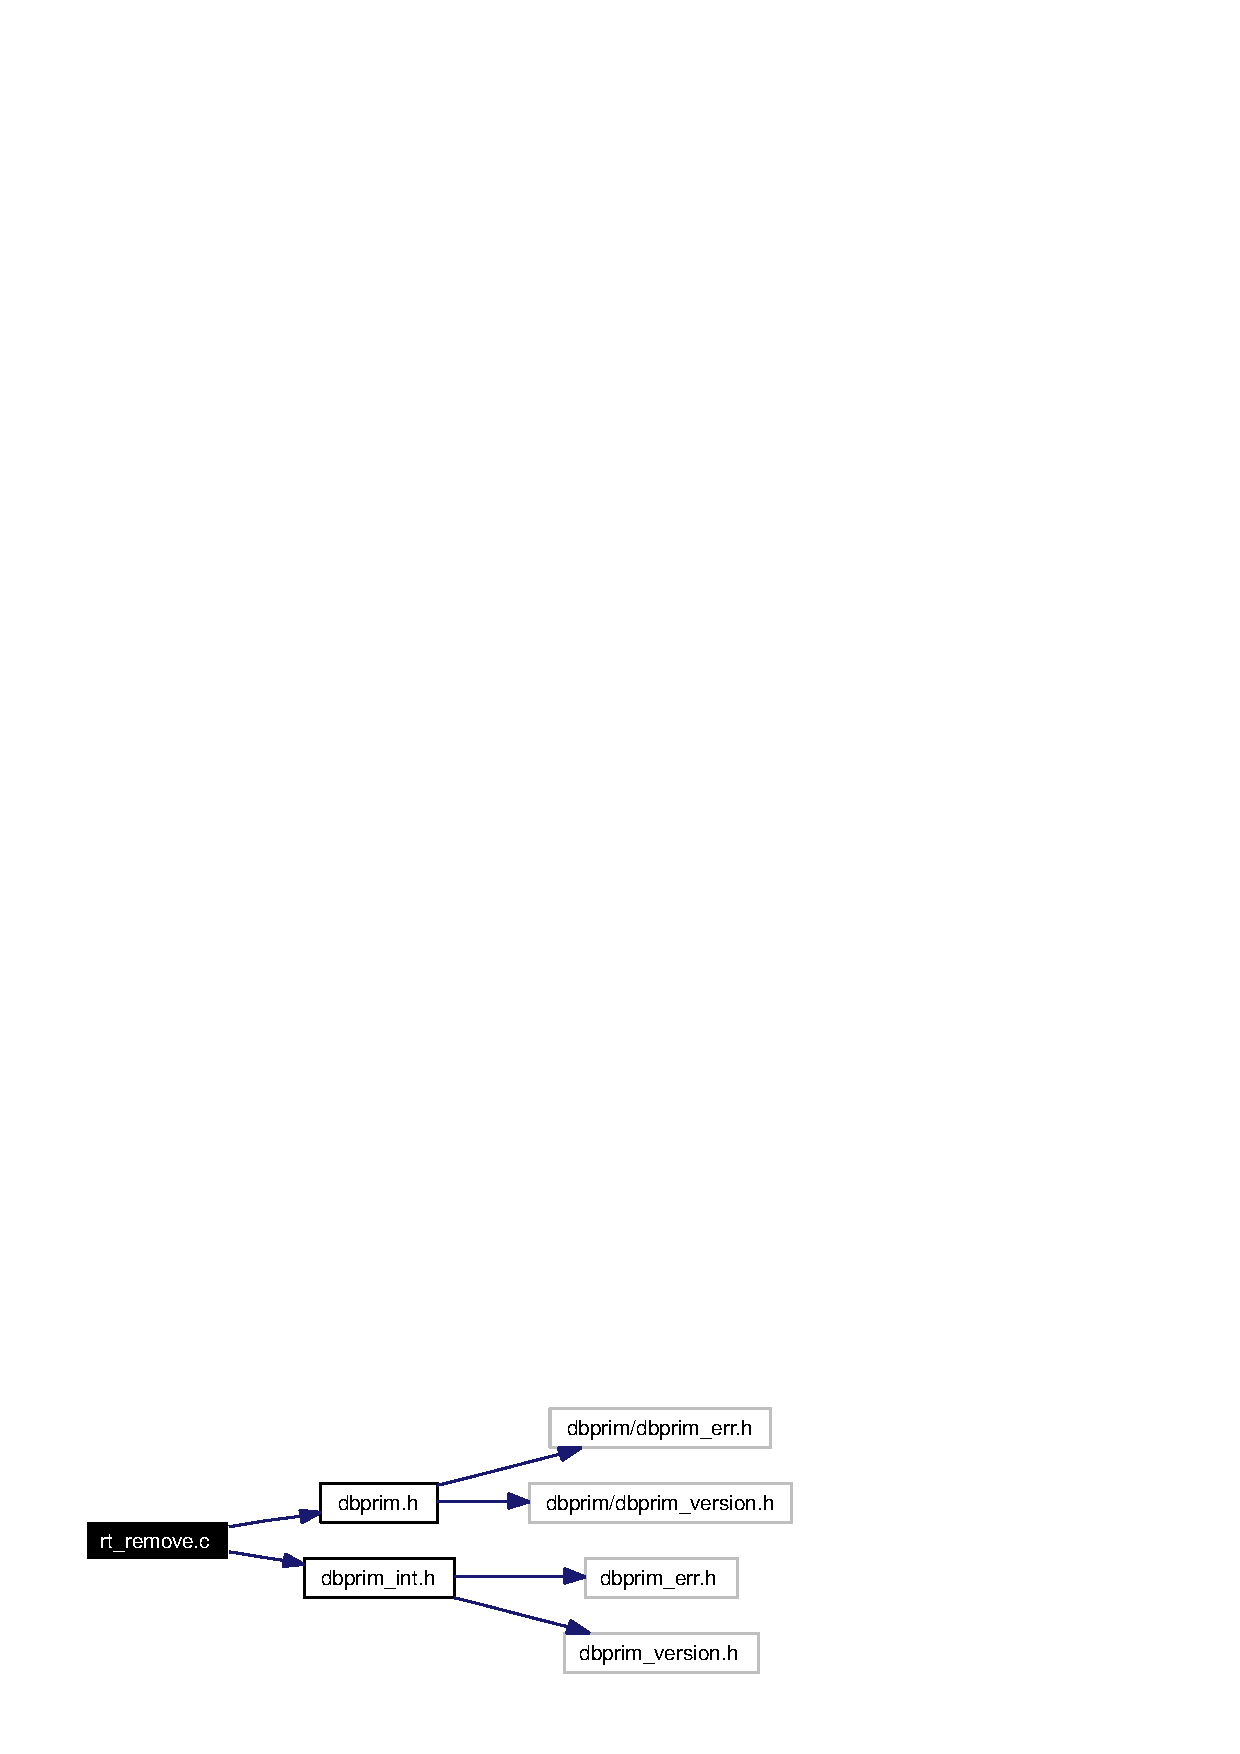
\includegraphics[width=192pt]{rt__remove_8c__incl}
\end{center}
\end{figure}
\subsection*{Defines}
\begin{CompactItemize}
\item 
\#define \hyperlink{group__dbprim__rbtree_ga46}{\_\-rn\_\-clear}(node)
\begin{CompactList}\small\item\em Clear a node. \item\end{CompactList}\item 
\#define \hyperlink{group__dbprim__rbtree_ga47}{\_\-rt\_\-update\_\-parent}(tree, node, new)
\begin{CompactList}\small\item\em Update a node's parent. \item\end{CompactList}\item 
\#define \hyperlink{group__dbprim__rbtree_ga48}{isleft}(par, n)
\begin{CompactList}\small\item\em Determine if node is a left child of its parent. \item\end{CompactList}\item 
\#define \hyperlink{group__dbprim__rbtree_ga49}{sel\_\-lr}(t, n)
\begin{CompactList}\small\item\em Select a child node based on a condition. \item\end{CompactList}\item 
\#define \hyperlink{group__dbprim__rbtree_ga50}{sibling}(par, n)
\begin{CompactList}\small\item\em Locate the sibling of a node. \item\end{CompactList}\item 
\#define \hyperlink{group__dbprim__rbtree_ga51}{l\_\-neph}(par, n)
\begin{CompactList}\small\item\em Locate \char`\"{}closer\char`\"{} nephew of a node. \item\end{CompactList}\item 
\#define \hyperlink{group__dbprim__rbtree_ga52}{r\_\-neph}(par, n)
\begin{CompactList}\small\item\em Locate \char`\"{}further\char`\"{} nephew of a node. \item\end{CompactList}\end{CompactItemize}
\subsection*{Functions}
\begin{CompactItemize}
\item 
unsigned long \hyperlink{group__dbprim__rbtree_ga9}{rt\_\-remove} (\hyperlink{struct__rb__tree__s}{rb\_\-tree\_\-t} $\ast$tree, \hyperlink{struct__rb__node__s}{rb\_\-node\_\-t} $\ast$node)
\begin{CompactList}\small\item\em Remove a node from a red-black tree. \item\end{CompactList}\end{CompactItemize}
